\documentclass[USenglish,twocolumn]{article}
\usepackage[utf8]{inputenc}
\usepackage[big,online]{dgruyter}
\usepackage{lmodern}
\usepackage{anyfontsize}
% \usepackage[sort&compress,square,numbers]{natbib}
\usepackage[backend=biber, citestyle=numeric, bibstyle=authoryear, hyperref=true, sorting=none, maxbibnames=99]{biblatex}
\usepackage{csquotes}
\usepackage{times}
\usepackage{bm}
\usepackage[nameinlink]{cleveref}
% \usepackage[toc, acronym, style=long3col, indexonlyfirst=true, nogroupskip=true]{glossaries}
\usepackage[backend=biber, citestyle=authoryear, bibstyle=authoryear, hyperref=true, sorting=none, maxbibnames=99]{biblatex}
\usepackage{csquotes}
\usepackage[nameinlink]{cleveref}
\usepackage{dsfont}

\usepackage{times}
\usepackage{xfrac}
\usepackage{bm}

\ifdefined\norm
  \renewcommand{\norm}[1]{\left\lVert#1\right\rVert_{\scriptscriptstyle 2}}
\else
  \newcommand{\norm}[1]{\left\lVert#1\right\rVert_{\scriptscriptstyle 2}}
\fi


\addbibresource{../literature/sources.bib}

% TODO: https://en.wikipedia.org/wiki/Non-negative_least_squares

% Report details: Max. 6 pages, composed of:
% • Summary
% • Introduction
% • Methods
% • Results
% • Future perspectives

\begin{document}
  %%%--------------------------------------------%%%
  %%% Please do not alter the following lines: %%%
  %%%--------------------------------------------%%%
  %\articletype{Proceedings}
  %\aop
  \DOI{10.1515/}
  \openaccess
  \pagenumbering{gobble}
  %%%--------------------------------------------%%%

  % \title{Performance optimization of the A549 electrophysiological cancer cell model and live simulation dashboard}
  \title{Improving runtime of the A549 electrophysiological cancer cell model from X to Y and live simulation dashboard}
  \runningtitle{Computational model of ion channel current}
  %\subtitle{Insert subtitle if needed}

  \author*[1]{Peter Waldert}
  \author[2]{Sonja Langthaler}
  % \author[2]{Third Author (Name Surname)}
  % \author[3]{Fourth Author (Name Surname)}
  \runningauthor{P.~Waldert et al.}

  \affil[1]{\protect\raggedright
    Institute of Health Care Engineering with European Testing Center for Medical Devices, Graz University of Technology, Graz, Austria, e-mail: peter.waldert@tugraz.at}
  \affil[2]{\protect\raggedright
    Institute of Health Care Engineering with European Testing Center for Medical Devices, Graz University of Technology, Graz, Austria}
  % \affil[2]{\protect\raggedright
  %   Institution (if same for both authors), city, country}
  % \affil[3]{\protect\raggedright
  %   Institution, city, country}

  \abstract{
    Through a reimplementation in Rust and numerical optimization approaches we were able to reduce the runtime of the A549 electrophysiological cancer cell model \cite{2021-A549-model} from X to Y.

    % Please insert your abstract here. Remember that online
    % systems rely heavily on the content of titles and abstracts to
    % identify articles in electronic bibliographic databases and search
    % engines. We ask you to take great care in preparing the abstract.
  }

  \keywords{Please insert your keywords here, separated by commas.}

  \maketitle

  \section{Introduction}
  Lung cancer is one of the most widespread pathologies worldwide and its internal workings, specifically those of individual A549 cells, are not well understood.
  Computational techniques can help with a better understanding of the behaviour of these cancer cells.
  We work with the A549 model introduced in \cite{2021-A549-model}, together with a calcium channel extension introduced in \cite{2024-calcium-channels}, reimplementing the model in the Rust programming language and performing a number of numerical optimizations such as adaptive timestepping.
  We also verify the model's performance in \textit{Floating} mode, as compared to an individual simulation of the estimated number of channels.
  We introduce a visualisation approach of the entire model in the form of a live simulation dashboard\footnote{\url{https://in-silico-cancer-cell.waldert.at/}}.
  The entire source code behind this simulation is freely available on GitHub\footnote{\url{https://github.com/MrP01/InSilicoCancerCell}}, and reusable through three different channels: the simulation interface (powered by WebAssembly), the Rust linkable library implementation and a Python package.
  These three interfaces all originate from the same source code and our aim behind a distribution in this ways is to make the simulation as accessible as possible.
  In order to find appropriate parameters for the model, an optimization procedure is performed.
  Multiple optimization approaches for the solution of the corresponding inverse problem (fitting model parameters to measurement data) are put in comparison.
  The measurements are obtained using a \textit{Patch-Clamp System}.

  \section{Methods}
  The computational model is as follows:
  A cell's membrane consists of multiple ion channels, categorized into $M \in \N$ different types (and therefore, sub-models).
  Each ion channel is represented in one of $N_{s, k} \in \N$ states, which, in physical terms, is related to a positional configuration of a protein within the ion channel.
  Only some states can be observed directly, and progress only depends on the one previous state.
  Hence, we are working with a Hidden Markov Model (HMM) where transitions between states are modelled probabilistically.
  For many ion channel categories, their transition probabilities are voltage or ion-concentration dependent.

  The whole cell current $I: T \to \R$ over time $t \in T \subset \R^+$ is then obtained as the sum of all individual channel contributions $I_k, k \in \{1, ..., M\}$ over $M \in \N$ channel types
  \begin{equation}
    I(t) := \sum_{k=1}^{M} N_k I_k(t) = \sum_{k=1}^{M} N_k g_k p_{o,k} \left(V(t)-E_k\right)\,,
  \end{equation}
  where $N_k$ is the number of channels of type $k \in \{1, ..., M\}$, $g_k$ is the respective ion channel's conductivity, $p_{o, k} \in [0, 1]$ is the probability of observing the channel in a state where an ion current can flow (``open states''), $V: T \to \R$ is the voltage across the membrane and $E_k \in \R^+$ the reversal potential.

  Within the simulation, we sample the state and current at discrete time points $T_{\rm meas} \subset T$, for example
  $$T_{\rm meas} := \left\{\sum_{i=0}^n (\Delta t)_i \;\bigg|\; n \in \N_0 \;\bigg|\; n < N_t\right\}$$
  for $N_t$ measurements with step size $(\Delta t)_n$, which may be chosen equally large for all $n \in \{0, ..., N_t - 1\}$.
  We will later adapt this time interval $(\Delta t)_n \in \R^+$ per simulation step based on a state change heuristic.

  The current measurements are then simply $\vec{I} := \left(I(t_0), I(t_1), ..., I(t_{N_t})\right)^T \in \R^{N_t}$.

  \subsection{Adaptive Timestepping}
  In order to accelerate the simulation in areas where there is little change to the dynamics, we choose an adaptive step size based on
  \begin{equation}
    (\Delta t)_n = (\Delta t)_{n-1} \left(\frac{\Delta^{\rm tol}}{\sum_{k=1}^{M} N_k \norm{s_{k,n} - s_{k,n-1}}_2}\right)^{1/2}\,,
  \end{equation}
  for all $n = 1, 2, ..., N_t - 1$.

  \subsection{Inverse Problem}
  When regarding the cell model as a whole, the number of ion channels $N_k$ per type $k$ may be put into a configuration vector $\vec{N} := (N_1, ..., N_M)^T \in \N^M$ and then the total simulated current $I$ sampled at measurement points $T_{\rm meas}$ can be expressed as a matrix-vector product
  \begin{equation}
    \vec{I} = \sum_{k=1}^{M} N_k \vec{I_k} = A \vec{N}\,,
    \label{eq:matrix-formulation}
  \end{equation}
  where $A \in \R^{N_t \times M}$ is the matrix of all current measurements per channel type.

  Given the individual ion channel type models' parameters, which we know from literature (cf. \Cref{table:channel-types}), the question that remains is how many channels there are of each type to fit the measurements.
  This problem can be solved using a number of optimization approaches.

  However, the formulation in \Cref{eq:matrix-formulation} also gives rise to a least-squares formulation, by projecting the measured current into the space of all individual channel currents.

  \begin{table}
    \caption{Ion Channel Types}
    \begin{tabular}{ll}
      \textbf{Channel Type} & \textbf{Reference}            \\
      \midrule
      Kv13                  & \cite{1998-potassium-channel} \\
      Kv31                  & \cite{1998-potassium-channel} \\
      Kv34                  & \cite{1998-potassium-channel} \\
      Kv71                  & \cite{1998-potassium-channel} \\
      KCa11                 & \cite{1998-potassium-channel} \\
      KCa31                 & \cite{1998-potassium-channel} \\
      Task1                 & \cite{1998-potassium-channel} \\
      CRAC1                 & \cite{1998-potassium-channel} \\
      TRPC6                 & \cite{1998-potassium-channel} \\
      TRPV3                 & \cite{1998-potassium-channel} \\
      CLC2                  & \cite{1998-potassium-channel} \\
    \end{tabular}
    \label{table:channel-types}
  \end{table}

  \subsection{Implementation Architecture}
  tbd

  \subsection{Live Simulation}
  tbd

  \begin{figure}
    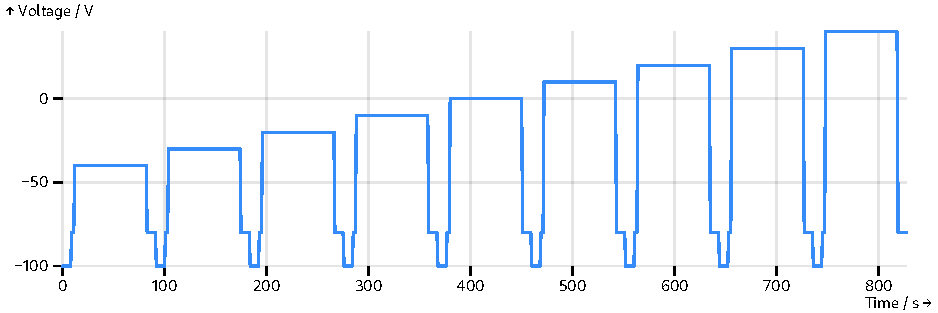
\includegraphics[width=\columnwidth]{../figures/results/voltage-protocol.pdf}
    \caption{Please insert your figure caption here.}
    \label{figure:voltage-protocol}
  \end{figure}

  \section{Results}
  \begin{figure}[h]
    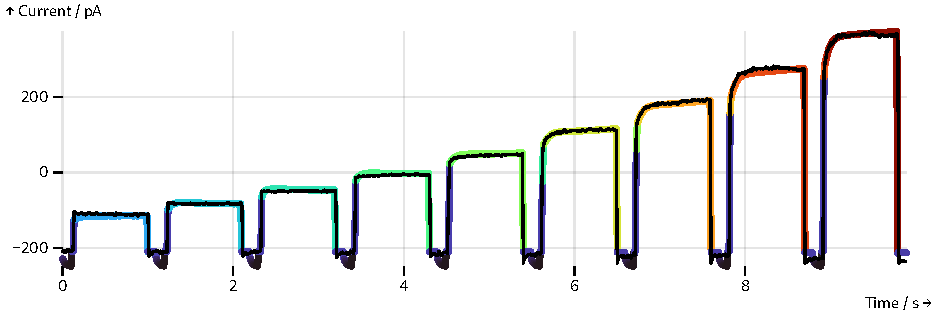
\includegraphics[width=\columnwidth]{../figures/results/full-simulation-current.pdf}
    \caption{Please insert your figure caption here.}
    \label{figure:full-simulation-current}
  \end{figure}
  \begin{figure}
    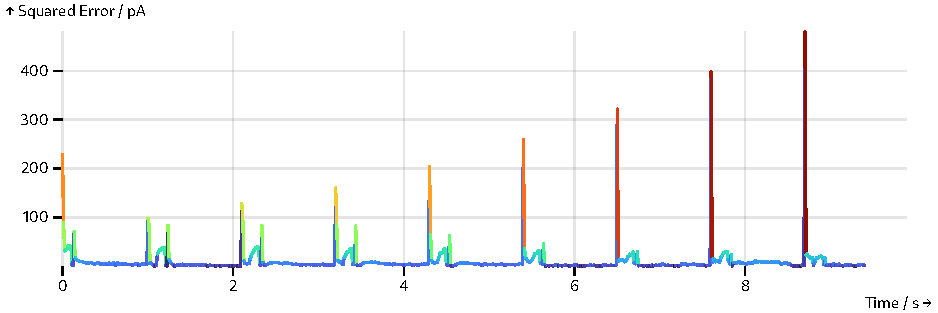
\includegraphics[width=\columnwidth]{../figures/results/simulation-error.pdf}
    \caption{Please insert your figure caption here.}
    \label{figure:simulation-error}
  \end{figure}

  \begin{table}
    \caption{Comparison of Optimization Approaches}
    \begin{tabular}{ll}
      \textbf{Algorithm}          & \textbf{Accuracy} \\
      \midrule
      Particle Swarm Optimization & 1                 \\
      Gradient Descent            & 2                 \\
      LBFGS                       & 3                 \\
      QR-based LSQ                & 4                 \\
      NNLS                        & 5                 \\
    \end{tabular}
    \label{table:optimization-comparison}
  \end{table}

  \begin{figure*}
    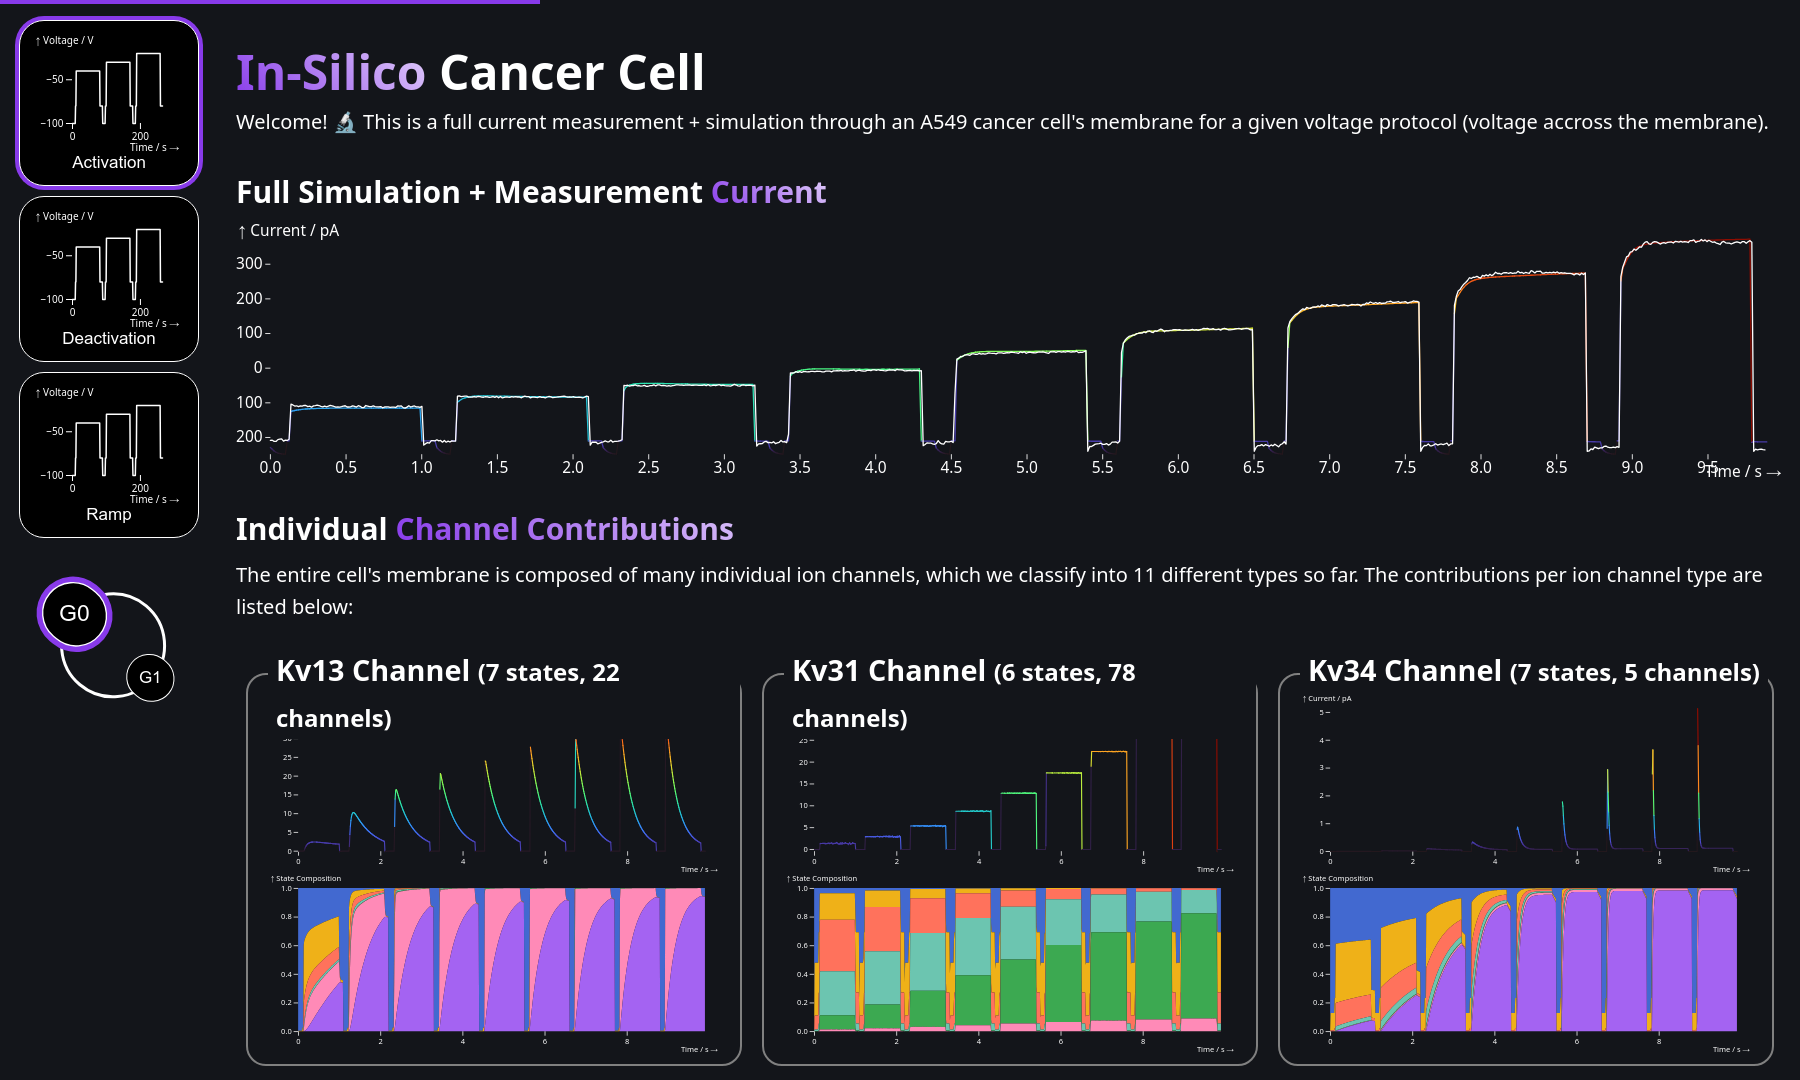
\includegraphics[width=2\columnwidth]{../figures/above-the-fold-screenshot.png}
    \caption{Please insert your figure caption here.}
    \label{figure:screenshot}
  \end{figure*}

  \section{Future Perspectives}
  Numerically, the stability of the simulation varies greatly with the time step state change tolerance $\Delta^{\rm tol}$, this could be improved using a higher-order integration scheme.
  Regarding the simulation dashboard, there are still many adjustments that could improve and enable further usage perspectives.

  \vspace{1cm}

  %\begin{acknowledgement}
  %\end{acknowledgement}

  \textsf{\textbf{Author Statement}}\\
  Research funding: This work was funded through a BioTechMed-Graz Lab Rotation Research Fellowship.
  Conflict of interest: Authors state no conflict of interest.
  Informed consent: Informed consent has been obtained from all individuals included in this study.
  Ethical approval: The research related to human use complies with all the relevant national regulations, institutional policies and was performed in accordance with the tenets of the Helsinki Declaration, and has been approved by the authors' institutional review board or equivalent committee.

  \printbibliography
\end{document}
